\section{Taylorformel \& lokale Extrema}
\textbf{Ziel:} Approximation durch Polynome im Mehrdimensionalen; Reduzierung auf 1-D Taylorapproximationen.

\begin{definition*}[Notation]
	Für $ \alpha = \left( \alpha_1, \dotsc, \alpha_n \right) \in \N _0^n $ (``Multiindex''):
	\[
		\left| \alpha \right| \coloneqq \left| \alpha_1 \right| + \dotsb + \left| \alpha_n \right| (= \alpha_1 + \dotsb + \alpha_n)
	\]
	\[
		\alpha! \coloneqq \alpha_1!\alpha_2!\dotsb\alpha_n!
	\]
\end{definition*}

Ist $ f $ $ \left| \alpha \right|  $-mal stetig differenzierbar, so sei
\[
	\partial ^{\alpha} f \coloneqq \partial_1^{\alpha_1} \dotsb \partial_n^{\alpha_n} f
\]
\textbf{Bedeutung:} $ \alpha_i $ entspricht wie oft man nach der $ i $-ten Variablen partiell ableitet.
Hierbei $ \partial_i^{\alpha_i} f \coloneqq \underbrace{\partial_i \left( \partial_i \dotsb \left( \partial_i f \right)  \right) }_{\alpha_i \text{-mal} } $.

\begin{theorem}
	Sei $ \Omega \subset \R ^n $ offen, $ f \Omega: \to \R  $ $ k $-mal stetig differenzierbar und $ x_0 \in \Omega $.
	Sei $ \xi \in \R ^n $ so, dass $ [x_0 , x_0 + \xi] \subset \Omega $.
	Dann ist $ g:[0, 1] \ni t \mapsto f(x_0 + t\xi) \in \R  $ $ k $-mal stetig differenzierbar und
	\[
		\frac{ \dd ^k g }{ \dd t^k } = \sum_{\left| \alpha \right| = k}^{} \frac{ k! }{ \alpha! } \left( \partial^{\alpha} f \right) (x_0 + t\xi) \xi^{\alpha} .
	\]
\end{theorem}
\begin{proof*}[Thm. \ref{5.1}]
	\[
		\forall k \in \N : \frac{ d^{k} g }{ \dd t^k } (t) = \sum_{i_1, \dotsc, i_k=1}^{n} \partial_{i_k} \dotsc \partial_{i_1} f(x_0 + t\xi) \xi_{i_1} \dotsb \xi_{i_k} 
	\]
	\begin{description}
		\item[$ k = 1 $:] 
			\[
				\frac{ \dd }{ \dd t } f(x_0 + t\xi) = \left< Df(x_0 + t\xi), \xi \right> = \sum_{i=1}^{n} \left( \partial_i f \right) \left( x_0 + t\xi \right) \xi_i
			\]
		\item[$ k - 1 \curvearrowright k $:]
			\begin{align*}
				\frac{ \dd ^k }{ \dd ^k } g &= \frac{ \dd }{ \dd t } \left( \frac{ \dd ^{k - 1} }{ \dd t^{k - 1}  } g(t) \right) \\
				~ & \overset{I.V.}{=} \frac{ \dd }{ \dd t } \sum_{i_1, \dotsc, i_{k - 1} =1}^{n} \partial_{i_{k - 1} } \dotsb \partial_{i_1} f\left( x_0 + t\xi \right) \cdot \xi_{i_1} \dotsb \xi_{i_{k - 1} } \\
				~ & = \sum_{i_1, \dotsc, i_{k - 1} =1}^{n} \partial_{i_{k - 1} } \dotsb \partial_{i_1} \left( \sum_{i_k=1}^{n} \partial_{i_k} f(x_0 + t\xi) \cdot \xi_{i_k}  \right) \xi_{i_1} \dotsb \xi_{i_k} \\
				~ &= \sum_{i_1, \dotsc, i_k=1}^{n} \partial_{i_k} \dotsb \partial_{i_1} f(x_0 + t\xi) \cdot \xi_{i_1} \dotsb \xi_{i_k}  \\
			\end{align*}
			\textbf{Kombinatorisch:} Wege des Satzes von Schwarz (Vertauschbarkeit partieller Ableitungen) treten hier partielle Ableitungen öfters auf.
			Speziell tritt $ \partial^{\alpha} f $ $ \frac{k!}{ \alpha! }  $ mal auf, und das zeigt die Behauptung. \qed
	\end{description}
\end{proof*}

\begin{theorem}[Taylor, mehrdimensional]
	Sei $ \Omega \subset \R ^n $ offen, $ x_0 \in \Omega $, $ \xi \in \R ^n $ mit $ [x_0, x_0 + \xi] \subset \Omega $.
	Sei $ f : \Omega \to \R  $ $ (k + 1) $-mal stetig differenzierbar.
	Dann $ \exists \theta \in [0, 1] $:
	\[
		f(x_0 + \xi) = \underbrace{ \sum_{\left| \alpha \right| \leq k}^{} \frac{ \partial ^{\alpha} f(x_0) }{ \alpha! } \xi^{\alpha} }_{\text{Taylorpolynom der Ordnung $ k $} } + \underbrace{ \sum_{\left| \alpha \right| =k + 1}^{} \frac{ \partial^{\alpha} f(x_0 + \theta \xi) }{ \alpha! } \xi^{\alpha} }_{\text{assoziiertes Restglied} }
	\]
\end{theorem}
\begin{proof*}[Thm \ref{5.2}]
	Setze
	\[
		g : [0, 1] \ni t \mapsto f(x_0 + t \xi) \in \R 
	\]
	$ k + 1 $-mal stetig differenzierbar $ \implies  $ [1-d Taylor] $ \implies \exists \theta \in [0, 1] $:
	\[
		g(1) = \sum_{m=0}^{k} \frac{ 1 }{ m! } g^{(m)} (0) + \frac{ g^{(k + 1)} (\theta) }{ (k + 1)! } .
	\]
	Aber
	\[
		\frac{g^{(m)} (0) }{ m! } = \frac{ 1 }{ m! } \sum_{\left| \alpha \right| =m}^{} \frac{ m! }{ \alpha! } \partial^{\alpha} f(x_0) \xi^{\alpha} = \sum_{\left| \alpha \right| =m}^{} \frac{ 1 }{ \alpha! } \partial^{\alpha} f(x_0) \xi^{\alpha} .
	\]
	\[
		\implies \sum_{m=0}^{k} \frac{ 1 }{ m! } g^{(m)} (0) = \sum_{m=0}^{k} \sum_{\left| \alpha \right| =m}^{} \frac{ 1 }{ \alpha! } \partial^\alpha f(x_0) \xi^\alpha = \sum_{\left| \alpha \right| \leq k}^{} \frac{ 1 }{ \alpha! } \partial ^{\alpha} f(x_0) \xi^{\alpha} .\qed
	\]
\end{proof*}

\begin{corollary}
	Sei $ \Omega $ offen, $ x_0 \in \Omega $, $ f : \Omega \to \R  $ $ k $-mal stetig differenzierbar.
	Dann haben wir bereits
	\[
		f(x_0 + \xi) = \sum_{\left| \alpha \right| \leq k}^{} \frac{ 1 }{ \alpha! } \partial^\alpha f(x_0) \xi^{\alpha} + o\left( \left| \xi \right| ^k \right) .
	\]
	mit $ \left| \xi \right| \searrow 0 $.
	\[
		\left[ \frac{ \left| f(x_0 + \xi) - \sum \left( \dotsc \right)  \right| }{ \left| \xi \right| ^k } \overset{\left| \xi \right| \searrow 0}{\longrightarrow} 0\right]
	\]
\end{corollary}
\begin{proof*}[Cor. \ref{5.3}]
	Nach Theorem \ref{5.2}
	\[
		\left| f(x_0 + \xi) = \sum_{\left| \alpha \right| \leq k}^{} \frac{ 1 }{ \alpha! } \partial^\alpha f(x_0) \xi^\alpha \right|
		=
		\left| \sum_{\left| \alpha \right| =k}^{} \frac{ \left( \partial^\alpha f(x_0 + \theta \xi) - \partial^\alpha f(x_0) \right) }{ \alpha! } \cdot \frac{ \xi^\alpha }{ \left| \xi \right| ^k }  \right| 
		\overset{\xi \searrow 0}{\longrightarrow} 0 \qed
	\]
\end{proof*}

\begin{note}
	Ist $ f $ in der Situation von Cor \ref{5.3} zweimal stetig differenzierbar, so gilt
	\[
		f(x_0 + \xi) = \underbrace{f(x_0)}_{\left| \alpha \right| = 0} + \underbrace{\left< Df(x_0), \xi \right>}_{\left| \alpha \right| = 1} + \underbrace{\frac{ 1 }{ 2 } \left< D^2 f(x_0) \xi, \xi \right> }_{\left| \alpha \right| = 2} + o \left( \left| \xi \right| ^2 \right) , \left| \xi \right| \searrow 0.
	\]
	
\end{note}

\textbf{Plan für heute:}
\begin{itemize}
        \item Notwendige \& hinreichende Kriterien für \textbf{Extrema} (bzw. lokale Ext.)
        \item ``Krümme'' von Graphen
\end{itemize}

\begin{definition}
        Sei $ \Omega \subset \R ^n $ offen \& $ f : \Omega \to \R  $ eine Funktion.
        Wir sagen, dass $ f $ in $ x_0 \in \Omega $
        \begin{itemize}
                \item ein \textbf{lokales Maximum} besitzt, falls $ \exists U \subset  \Omega $ offen $ \forall x \in U : f(x) \leq f(x_0) $.
                \item ein \textbf{lokales Minimum} besitzt, falls $ \exists U \subset  \Omega $ offen $ \forall x \in U : f(x) \geq f(x_0) $.
                \item ein \textbf{lokales Extremum}, falls in $ x_0 $ ein lokales Maximum/Minimum vorliegt
        \end{itemize}

\end{definition}

\begin{theorem}
        Sei $ \Omega \subset \R ^n $ offen, $ f: \Omega \to \R  $ eine partiell differenzierbare Funktion.
        Hat $ f $ in $ x_0 $ ein lokales Extremum, so $ \nabla f (x_0) = \left( \partial_1 f(x_0), \dotsc, \partial_n f(x_0) \right) = (0, \dotsc, 0) $
\end{theorem}
\begin{proof*}[Thm. \ref{5.6}]
        Sei $ U \subset \Omega $ wie in dder Definition des lokalen Extremum, \OE{} lokales Maximum.
        Dann $ \exists  \varepsilon > 0 : \forall t \in \left( -\varepsilon , \varepsilon  \right) : \forall j : x_0 + t e_j \in U $.
        Nun hat also für jedes $ j \in \left\{ 1, \dotsc, n \right\}  $ die Funktion $ g_j (t) \coloneqq f(x_0 + t e_j) $ ein lokales Maximum in $ t = 0 $;
        $ g_j : \left( -\varepsilon , \varepsilon  \right) \to \R  $.
        Damit nach Ana 1: $ 0 \overset{!}{=}g_j^\prime (0) $, aber $ g_j^\prime (t) = \left< D f(x_0 + te_j), e_j \right>  $ \& daher $ g_j^\prime (0) = \partial_j f(x_0) $.\qed
\end{proof*}

\textbf{Ziel:} Hinreichende Bedingung
\begin{itemize}
        \item $ x \mapsto x^2 $\\
		\begin{tikzpicture}
			\begin{axis}[
				xmin= -2, xmax= 2,
				ymin= -4, ymax = 4,
				axis lines = middle,
				xtick = { -1, 1 },
				ytick = { -3, -1, ..., 3 },
				extra x ticks = { -2, -1, ..., 2 },
				extra y ticks = { -4, -3, ..., 4 },
				extra x tick labels = {},
				extra y tick labels = {},
				height = 8cm,
				width = 8cm,
			]
				\addplot[domain=-2:2, samples=100]{x^2};
			\end{axis}
		\end{tikzpicture}\\
		``pos. gekrümmt''
        \item $ x \mapsto - x^2 $\\
		\begin{tikzpicture}
			\begin{axis}[
				xmin= -2, xmax= 2,
				ymin= -4, ymax = 4,
				axis lines = middle,
				xtick = { -1, 1 },
				ytick = { -3, -1, ..., 3 },
				extra x ticks = { -2, -1, ..., 2 },
				extra y ticks = { -4, -3, ..., 4 },
				extra x tick labels = {},
				extra y tick labels = {},
				height = 8cm,
				width = 8cm,
			]
				\addplot[domain=-2:2, samples=100]{-x^2};
			\end{axis}
		\end{tikzpicture}\\
		``neg. gekrümmt''
\end{itemize}

\begin{itemize}
	\item Für $ x \mapsto ax^2 $ definiert $ a \in \R  $ das Krümmungsverhalten
\end{itemize}
Für \textsc{Multi-Dim.:} Substitute von $ x \mapsto ax^2 $ sind die quadratischen Formen: $ q : \R ^n \ni x \mapsto  \left< A x, x \right> \in \R  $, wobei $ A \in \R ^{n \times n}  $.

\begin{example}
	Sei $ A = E_n  $ ($ (n\times n) $-Einheitsmatrix), \OE{} für $ n = 2 $.
	Dann
	\[
		q : \R ^n \ni x \mapsto \left\| x \right\| _2^2 = x_1^2 + x_2^2 + \dotsb x_n^2.
	\]
	\[
		\tilde q : \R ^n \ni x \mapsto -\left\| x \right\| _2^2 \text{ (zu $ A = -E_h $)} 
	\]
	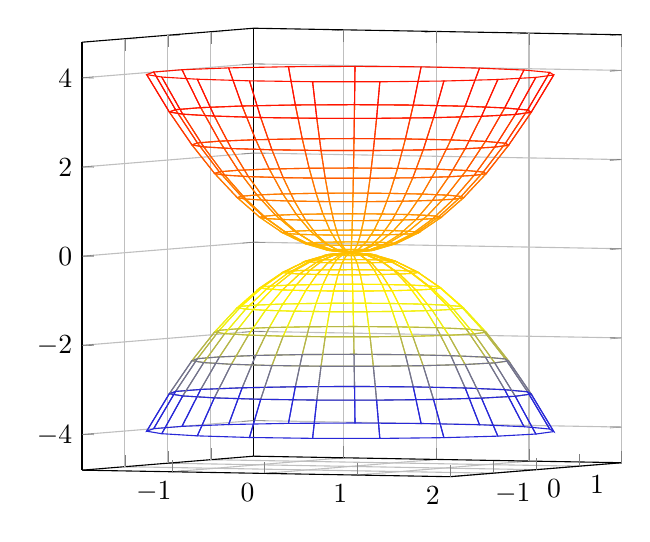
\begin{tikzpicture}
                \begin{axis}[
                        domain = 0:2,
                        samples = 10,
                        y domain = 0:2*pi,
                        samples y = 20,
                        grid,
			plot box ratio = 1 1 16,
                        %height = 8cm,
			%hide axis,
			]
			\addplot3[
				mesh,
				%smooth,
				trig format plots=rad,
				]
				({x * cos(y)}, {x * sin(y)}, {-x^2});
			\addplot3[
				mesh,
				%smooth,
				trig format plots=rad,
				]
				({x * cos(y)}, {x * sin(y)}, {x^2});
			%\addplot3[surf] {(x^2 + y^2)};
                \end{axis}
        \end{tikzpicture}
\end{example}

\begin{definition}
	Eine symmetrische Matrix $ A \in \R _{\text{sym} } ^{n \times n}  $ (also $ a_{ij} = a_{ji}  $) heißt
	\begin{itemize}
		\item pos. definit, falls $ \forall x \in \R ^n \setminus \left\{ 0 \right\} : \left< Ax, x \right> > 0 $.
		\item pos semidefinit, falls $ \forall x \in \R ^n \setminus \left\{ 0 \right\} : \left< Ax, x \right> \geq  0 $.
		\item neg. definit, falls $ \forall x \in \R ^n \setminus \left\{ 0 \right\} : \left< Ax, x \right> < 0 $.
		\item neg. semidefinit, falls $ \forall x \in \R ^n \setminus \left\{ 0 \right\} : \left< Ax, x \right> \leq  0 $.
		\item undefinit, falls keine der obigen Bedingungen erfüllt sind.
	\end{itemize}
\end{definition}

\begin{note}
	Ang., $ A \in \R _{sym} ^{n \times n}  $ erfüllt $ \forall x \in B_{\varepsilon}(0) : \left< Ax, x \right> \geq  0 $.
	Für $ y \in \R ^n \setminus \left\{ 0 \right\}  $ sei
	\[
		x_{\varepsilon } \coloneqq \frac{ \varepsilon }{ 2 } \frac{ y }{ \left\| y \right\| _2 } .
	\]
	Dann
	\[
		x_{\varepsilon } \in B_{\varepsilon}(0) \& \underbrace{ \left< Ax_\varepsilon , x_\varepsilon  \right> }_{ \underbrace{ \frac{ \varepsilon ^2}{ 4 } \frac{ 1 }{ \left\| y \right\| _2^2 } }_{>0} \left< Ay, y \right>  } \geq 0
	\]
\end{note}

\begin{theorem}
	Sei $ \Omega \subset \R ^n $ offen, $ f: \Omega \to \R  $ zweimal stetig differenzierbar und $ x_0 \in \Omega $ mit $ Df(x_0) = 0 $.
	Dann gilt: Ist
	\begin{enumerate}[label=(\roman*)]
		\item $ D^2f(x_0) $ (bzw. $ Hf(x_0) $) \textbf{pos. definit}, so hat $ f $ in $ x_0 $ ein lokales Minimum
		\item $ D^2f(x_0) $ (bzw. $ Hf(x_0) $) \textbf{neg. definit}, so hat $ f $ in $ x_0 $ ein lokales Maximum
		\item Ist $ D^2f(x_0) $ $ (Hf(x_0)) $ indefinit, so liegt kein lokales Extremum in $ x_0 $ vor.
	\end{enumerate}
\end{theorem}
\begin{proof*}[Thm. \ref{5.10}]
	Nur (i), (ii), (iii) analog.
	Nach Tayorentwicklung zu Ornung 2 schreibe
	\[
		f(x) = f(x_0) + \left< Df(x_0), x - x_0 \right> + \frac{ 1 }{ 2 } \left< D^2 f(x_0) (x - x_0), (x - x_0) \right> + r(x) \left\| x - x_0 \right\| _2^2
	\]
	für alle $ x \in \omega $ \& $ \lim_{x \to x_0} \left| r(x) \right| = 0 $.
	Definiere $ A \coloneqq D^2 f(x_0) $. Betrachte
	\[
		q : x \mapsto \left< Ax, x \right>.
	\]
	Dann ist $ q $ stetig, und nimmt $ \mathdollar ^{n - }  $ sin Minimum an ($ \mathdollar ^{n - 1}  $ kompakt).
	Sei  nun $ \varepsilon \coloneqq \min_{\mathdollar^{n - 1} } q $, $ \mathdollar^{n - 1} = \left\{ x \in \R ^n: \left\| x \right\| _2 = 1 \right\}  $.
	Nun ist $ A $ pos. definit, also $ \varepsilon > 0 $.
	Dann, z.B. mit Bem. \ref{5.9}: $ \left< Ay, y \right> \geq \varepsilon \left\| y \right\| _2^2 $ für alle $ y \in \R ^n $.
	Denn $ \forall y \neq 0 : \frac{ y }{ \left\| y \right\| _2 } \in \mathdollar^{n - 1}  $, also $ \left< A \frac{ y }{ \left\| y \right\| _2 } , \frac{ y }{ \left\| y \right\| _2 }  \right> \geq \varepsilon  $.
	Weiter $ \exists \delta > 0 : \forall x \in B_{\delta}(x_0) : \left| r(x) \right| < \frac{ \varepsilon }{ 2 }  $.
	Hiermit 
	\begin{align*}
		\forall x \in B_{\delta}(x_0) : f(x) &= f(x_0) + \underbrace{\left< A(x - x_0), (x - x_0) \right> }_{\geq \varepsilon \left\| x - x_0 \right\| _2^2} + r(x) \left\| x - x_0 \right\| _2^2 \\
		~ &\geq f(x_0) + \frac{ \varepsilon }{ 2 } \left\| x - x_0 \right\| _2^2 - \underbrace{\left| r(x) \right| }_{\leq  \frac{ \varepsilon }{ 2 } } \cdot \left\| x - x_0 \right\| _2^2 \\
		~ & \geq f(x_0) + \frac{\varepsilon }{ 2 } \left\| x - x_0 \right\| _2^2 - \frac{\varepsilon }{ 2 } \left\| x - x_0 \right\| _2^2 = f(x_0).\qed
	\end{align*}
\end{proof*}

Zum Überprüfen der (pos.) Definitheit: Hauptminoren für $ A = (a_{ij} )_{i,j = 1}^n  $ 
\[
	\left| A_1 \right| = a_{11}.
\]
\[
	\left| A_2 \right| = \det \begin{pmatrix} a_{11} & a_{12} \\ a_{21} & a_{22} \end{pmatrix} 
\]
\[
	\left| A_k \right| = \det \begin{pmatrix} a_{11} & \hdots & a_{1k} \\ \vdots & & \vdots \\ a_{k1} & \hdots a_{kk}  \end{pmatrix} \text{``$ k $-te Hauptminore''} 
\]

\begin{theorem}[Hirwitz]
	Sei $ A \in \R _{sym} ^{n \times n}  $. $ A $ ist
	\begin{enumerate}[label=(\roman*)]
		\item pos. definit, falls alle Hauptminoren $ > 0 $ sind.
		\item (neg. definit) Die Hauptminoren wechseln mit neg. Vz beginnend ihre Vorzeichen:
			$ \left| A_1 \right| <0, \left| A_2 \right| > 0, \left| A_3 \right| < 0, \dotsc $
			\begin{itemize}
				\item $ -I $: $ \left| A_1 \right|  = -1 $, $ \left| A_2 \right| = \det \begin{pmatrix} -1  & 0 \\ 0 & -1 \end{pmatrix} = 1, \dotsc $ 
			\end{itemize}
	\end{enumerate}
\end{theorem}

\begin{example}
	$ f: \R ^2 \to \R , f(x, y) \coloneqq x^3 + xy^2 + x^2 - y^2 $.\\
	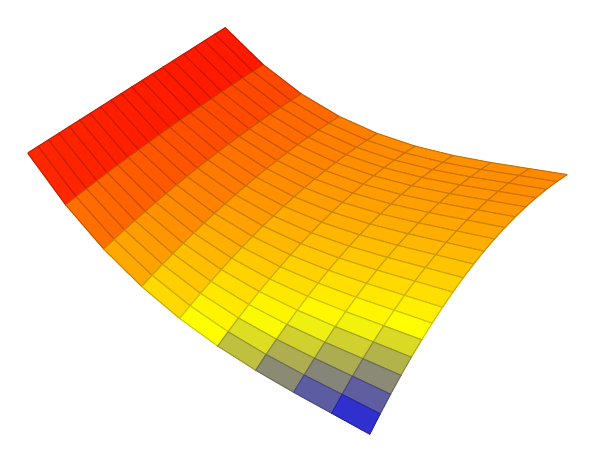
\begin{tikzpicture}
                \begin{axis}[
			view/h=-150,
                        domain = -0.5:1,
                        samples = 10,
                        y domain = -0:1.5,
                        samples y = 20,
                        grid,
                        %height = 8cm,
			hide axis,
			]
			\addplot3[surf] {(x^3 + x * y^2 + x^2 - y^2)};
                \end{axis}
        \end{tikzpicture}\\
	\textbf{Frage:} Wo lokale Extrema?
	\[
		\nabla f(x, y) = \begin{pmatrix} 3x^2 + y^2 + 2x \\ 2(x - 1)y \end{pmatrix} \overset{!}{=} 0
	\]
	$ \implies x = 1 \vee y = 0 $
	\[
		\nabla (x, y) = \begin{pmatrix} 5 + y^2 \\ 0 \end{pmatrix} \neq \begin{pmatrix} 0 \\ 0 \end{pmatrix}
	\]
	$ \implies  $ \OE{} $ y = 0 $ $ \implies 3x^2 + 2x \overset{!}{=} 0 \implies  x = - \frac{ 2 }{ 3 } \vee x = 0 $.
	\textbf{Kritische Punkte:} $ \xi_1 \coloneqq (0, 0), \xi_2 = \left( - \frac{ 2 }{ 3 } , 0 \right)  $.
	\[
		D^2 f (x, y) = \begin{pmatrix} 6x + 2 & 2y \\ 2y & 2(x - 1) \end{pmatrix} .
	\]
	Dann
	\[
		D^2f(\xi_1) = \begin{pmatrix} 2 & 0 \\ 0 & -2 \end{pmatrix} = A,
	\]
	$ \left| A_1 \right| = 2 > 0, \left| A_2 \right| < 0 $.
	Aber $ A $ ist indefint:
	$ \left< A \begin{pmatrix} 1 \\ 0 \end{pmatrix} , \begin{pmatrix} 1 \\ 0 \end{pmatrix}  \right> > 0$, $ \left< A \begin{pmatrix} 0 \\ 1 \end{pmatrix} , \begin{pmatrix} 0 \\ 1 \end{pmatrix}  \right> <0 $.
	Also nach Thm. \ref{5.10} c) \textbf{kein} lokales Extremum.
	\[
		(x, y) = \left( - \frac{ 2 }{ 3 } , 0 \right) , D^2 f\left( x, y \right) = \begin{pmatrix} -2 & 0 \\ 0 & - \frac{ 10 }{ 3 }  \end{pmatrix} 
	\]
	Eintrag links oben neg., $ \det D^2f(x, y) = \frac{ 20 }{ 3 } > 0 $. Also ist $ D^2 f(x, y) $ nach Hurwitz \textbf{neg. definit} $ \implies  $ bei $ \left( -\frac{ 2 }{ 3 } , 0 \right)  $ hat $ f $ ein \textbf{lok. Maximum}.
	Dies ist \textbf{kein} globales Maximum, denn für $ (x, 0): f(x, 0) = x^3 + x^2 \overset{x \to \infty}{\longrightarrow} \infty $.

	\begin{itemize}
		\item \textbf{Affensattel:} $ f(x, y) = x^3 - 3xy^2 $ 
			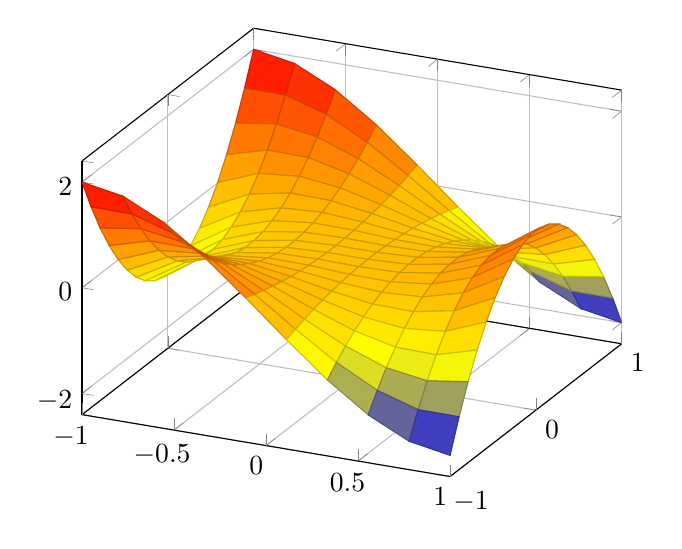
\begin{tikzpicture}
				\begin{axis}[
					domain = -1:1,
					samples = 10,
					y domain = -1:1,
					samples y = 20,
					grid,
					%height = 8cm,
					%hide axis,
					]
					\addplot3[surf] {(x^3 - 3 * x * y^2)};
				\end{axis}
			\end{tikzpicture}\\
			\[
				\nabla f(x, y) = \begin{pmatrix} 3x^2 - 3y^2 \\ -6xy \end{pmatrix} \overset{!}{=} \begin{pmatrix} 0 \\ 0 \end{pmatrix} 
			\]
			$ \implies (x, y) = (0, 0) $ 
			\[
				D^2 f(x, y) = \begin{pmatrix} 6x & -6y \\ -6y & -6x \end{pmatrix} \overset{(x, y) = (0, 0)}{=} \begin{pmatrix} 0 & 0 \\ 0 & 0 \end{pmatrix} \to \text{kein lok. Extremum} 
			\]
	\end{itemize}
	
\end{example}

